\chapter{Fundamentação Teórica}

Este capítulo aborda em detalhes os principais conceitos e tecnologias que fundamentam o projeto, incluindo temas como Internet das Coisas (\textit{IoT}), Sistemas Distribuídos, 
Redes de Computadores (Wi-Fi e Bluetooth), protocolo de comunicação HTTP, desenvolvimento de \textit{software} para a plataforma Android, características do microcontrolador ESP32, monitoramento de 
exposição ao monóxido de carbono e trabalhos relacionados. Todos os tópicos citados possuem papel crucial no desenvolvimento da solução proposta no trabalho de conclusão de curso. Dessa forma, o
objetivo é fornecer ao leitor uma visão abrangente das competências desenvolvidas em sua execução.

\section{Internet das Coisas}

O termo \textit{Internet das Coisas} (\textit{IoT}, da expressão em inglês \textit{Internet of Things}) foi utilizado primeiramente em 1999 pelo então pesquisador do \textit{Massachusetts Institute of Technology} (MIT) Kevin Asthon, em 
uma apresentação na Procter \& Gamble (P\&G) sobre a tecnologia do \textit{Radio Frequency Identification} (RFID). O RFID é uma tecnologia utilizada para a identificação e rastreamento de objetos, animais ou pessoas 
via ondas de rádio. Portanto, Asthon pontuou a possibilidade de utilizar tal ferramenta para gerenciar a cadeia de suprimentos da empresa, pois sua capacidade de ler vários emissores simultaneamente, sem a necessidade de linha de visão direta entre o leitor 
e a tag (ao contrário do códigos de barras) torna o monitoramento de cada produto nos distintos pontos de transporte mais preciso. A ideia do autor consiste na responsabilidade dos próprios objetos sobre a coleta de dados
e reação aos estímulos do ambiente, pois os computadores podem reduzir custos com base em decisões pautadas na observação do mundo exterior \cite{iot-first-definition}.

\textit{IoT} possui muitas definições. Embora não haja um consenso para uma definição única, podemos discutir sobre seu impacto na sociedade atual e aspectos importantes que toda solução na área possui. No livro \textit{The Internet  of Things}, escrito por 
Samuel Greengard, o tema é abordado como um evento disruptivo, onde a linha que separa o humano e a tecnologia se torna cada vez menos visível, porém o texto aborda não somente a capacidade de conexão entre as máquinas, e sim a autonomia 
e ``inteligência'' crescente dos sistemas embarcados \cite[pp. 17]{book-iot}. Essa visão de tecnologia integrada no cotidiano é o conceito que o autor Mark Weiser aborda no seu artigo, denominado \textit{The Computer for the 21st Century}. A computação ubíqua 
é o processo de tornar os computadores ``invisíveis'' aos nossos olhos, desenvolvendo a comunicação com tais ferramentas o mais próximo possível da forma humana, ou seja, o dispositivo tem conexão com a rede e responde aos estímulos do usuário por 
interfaces naturais, por exemplo, a fala e gestos com as mãos \cite{ubiquitous-computing}.

Portanto, o significado mais comum de \textit{IoT} talvez seja o de dispositivos eletrônicos conectados na internet, permitindo 
enviar e receber dados do ambiente real. No entanto, apenas conectar dispositivos não é uma solução em Internet das Coisas, pois essa 
área envolve o uso de protocolos de comunicação, eletrônica de baixo consumo energético, plataformas em nuvens e outras inúmeras 
áreas do conhecimento. Os dados coletados de sensores atuam como combustível para a execução de um fluxo de tomada de decisão \cite{iot-cycle}. 

\begin{figure}[ht]
    \centering
    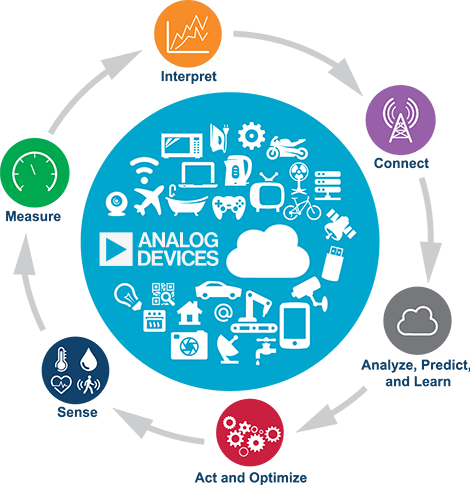
\includegraphics[width=.45\textwidth]{img/iot-cycle.png}
    \caption{Ciclo de IoT. Fonte: \cite{iot-cycle}}\label{figIoTCycle}
\end{figure}

Atualmente, a coleta de dados e o uso de ferramentas de análise são os principais recursos de empresas competitivas no gerenciamento de suas atividades. Com o 
avanço da área de telecomunicações, as organizações têm potencial de transformar grandes volumes de dados em \textit{insights} poderosos, que orientam a tomada de 
decisões da equipe de gestão, em busca de eficiência. Portanto, a Internet das Coisas representa uma tendência forte e disruptiva na sociedade.

\section{Sistemas Distribuídos}

``Um sistema distribuído é aquele no qual os componentes localizados em computadores interligados em rede se comunicam e coordenam suas ações apenas passando mensagens.'' \cite[pp. 1]{sistemas-distribuidos-coulouris2013}.
A definição do autor leva em conta dois importantes fatores: o primeiro é a comunicação via rede de computadores, e o segundo está relacionado ao provisionamento de um serviço.
O mundo atual oferece inúmeros exemplos de sistemas distribuídos atuando no desenvolvimento socioeconômico. A modalidade de educação à distância \cite{mec-ead}, por exemplo, utiliza serviços 
web e compartilhamento multimídia para levar o ensino de qualidade a pessoas fisicamente distantes dos grandes centros de ensino ou sem infraestrutura escolar adequada, como em comunidades 
ribeirinhas e regiões rurais. Outro caso é o da telemedicina, onde os sistemas distribuídos permitem que consultas virtuais seguras sejam realizadas com 
especialistas em diversas áreas da medicina, facilitando o exame e diagnóstico de doenças na população residente em regiões de difícil acesso \cite{telemedicina}. A preservação do meio ambiente 
também se beneficia do uso de sistemas distribuídos, pois o ``Curupira'' é um exemplo de sistema de monitoramento para áreas de floresta fechada com o intuito de detectar ameaças de desmatamento. O projeto utiliza 
uma rede de sensores que enviam sinais de perigo para um roteador central, com área de cobertura de 15 km \cite{curupira}.

Portanto, sistema distribuído tem foco no compartilhamento de recursos. Na web, a implementação de arquitetura mais comum é o modelo cliente-servidor, pois
um número grande de aplicações utiliza essa premissa, por exemplo, plataformas de redes sociais, jogos online e serviços bancários.
Ao nível do Sistema Operacional, a comunicação entre processos executados em diferentes computadores interligados em rede é essencial para o gerenciamento e acesso aos recursos distribuídos.
Nesse contexto, um cliente, que pode ser um processo ou aplicativo, realiza uma solicitação ao servidor para acessar ou manipular um recurso, como arquivos, impressoras, ou mesmo capacidade de processamento. O servidor, 
ao receber essa solicitação, desencadeia uma série de operações internas, que podem incluir desde a autenticação do cliente até a busca de dados em um banco de dados distribuído. Em seguida, o servidor 
retorna o resultado ao cliente em espera, completando o ciclo de comunicação do tipo requisição e resposta \cite[pp. 16]{sistemas-distribuidos-coulouris2013}.

Outro conceito importante é o de tolerância à falha. Essa característica permite um sistema continuar operando mesmo diante da falha de um ou mais 
componentes internos. Ou seja, é a capacidade do sistema distribuído em identificar e isolar seus defeitos a fim de preservar o seu estado global, pois essa propriedade é 
importante em sistemas críticos como, por exemplo, em sistemas de controle aéreo ou financeiros, onde interrupções podem levar a graves consequências e prejuízos \cite[pp. 528]{sistemas-distribuidos-coulouris2013}.

\section{Redes de Computadores}

``A internet é um subsistema de comunicação único que fornece comunicação entre todos os hosts conectados a ela'' \cite[pp. 96]{sistemas-distribuidos-coulouris2013}. Portanto, uma rede de computadores 
permite que sistemas se comuniquem e troquem mensagens por protocolos, sendo estes um conjunto específico de regras para o envio e recebimento de dados. No contexto de redes locais sem fio, esta seção trata de duas 
implementações utilizadas no sistema BURI: Wi-Fi e Bluetooth. A primeira tecnologia tem aplicação em redes locais de velocidade alta em residências e locais públicos. Porém, a segunda trata-se de uma comunicação direta entre dois 
dispositivos e possui alcance muito menor, assim como baixo consumo de energia.

Por se tratar de um sistema crítico, visto que envolve detecção de gases asfixiantes, o sistema proposto deve ser tolerante à falha. Portanto, a rede Wi-Fi tem como papel o acesso à Internet e armazenamento do histórico de dados, enquanto o 
Bluetooth realiza a transmissão de dados em tempo real para o dispositivo mais próximo, ou seja, o celular do usuário com o aplicativo móvel.

\subsection{Wi-Fi}

A rede Wi-Fi, inicialmente designada como a \textbf{LAN sem fio IEE 802.11}, é uma tecnologia de comunicação 
que permite aos hospedeiros sem fio acesso a redes maiores por uma infraestrutura baseada em pontos de acesso (\textit{access point} - AP). Em termos 
de arquitetura, o hospedeiro móvel realiza uma varredura e encontra APs disponíveis através do envio periódico de quadros de sinalização por parte dos pontos, contendo o identificador da 
rede SSID (do inglês, \textit{Service Set Identifier}) e o endereço MAC do AP. Em seguida, o usuário escolhe um desses pontos para 
se associar, solicitando entrada na sub-rede e obtendo um IP \cite{redeskurose2010}. 

\begin{figure}[ht]
    \centering
    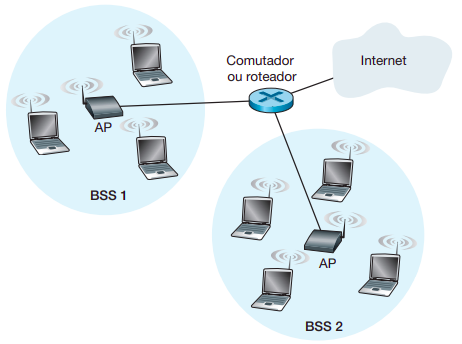
\includegraphics[width=.42\textwidth]{img/wifi-design.png}
    \caption{Arquitetura de rede LAN IEE 802.11. Fonte: \cite{redeskurose2010}}\label{figWifi}
\end{figure}

Apesar das vantagens, como a flexibilidade de conexão na internet de vários dispositivos sem a necessidade 
de fio e alta banda de transmissão, esse tipo de rede sem fio também possui desafios técnicos. Entre as diferenças 
em comparação com um enlace com fio, temos: redução na intensidade do sinal eletromagnético devido aos obstáculos físicos 
como paredes, portas e eletrodomésticos; interferência com outras ondas de rádio no meio de propagação, pois o ruído de fontes
externas impacta na taxa de transmissão e banda do canal de comunicação; corrupção dos bits do pacote transmitido, gerando 
o uso de mecanismos de códigos de correção. Por exemplo, a relação sinal-ruído (SNR) é um valor numérico em decibéis (dB) que informa 
ao receptor o quão fácil ele consegue retirar a informação do sinal recebido com ruído \cite[pp. 408]{redeskurose2010}.

\subsection{Bluetooth}

``Bluetooth é uma tecnologia de rede pessoal sem fio que surgiu a partir da necessidade de
conectar telefones móveis a PDAs, notebooks e outros equipamentos pessoais sem fios'' \cite[pp. 138]{sistemas-distribuidos-coulouris2013}. A tecnologia
possui como restrições o baixo consumo de energia e uso na comunicação entre dispositivos portáteis, pois, diferente do Wi-Fi, o Bluetooth 
necessita de menor largura de banda e alcance de transmissão. No começo, o padrão realizava transporte de voz no meio digital com dispositivos de baixo consumo. Atualmente, seu uso em todo o mundo é para conectar 
dispositivos eletrônicos como mouses sem fio, teclados, fones de ouvido e demais dispositivos móveis. A conexão ocorre pelo ``emparelhamento'', processo onde dois dispositivos 
trocam informações, como a chave de segurança do outro ou a comparação de número (PIN), e salvam os dados para o uso em conexões futuras \cite{blueetoothIntel}. 

\begin{figure}[ht]
    \centering
    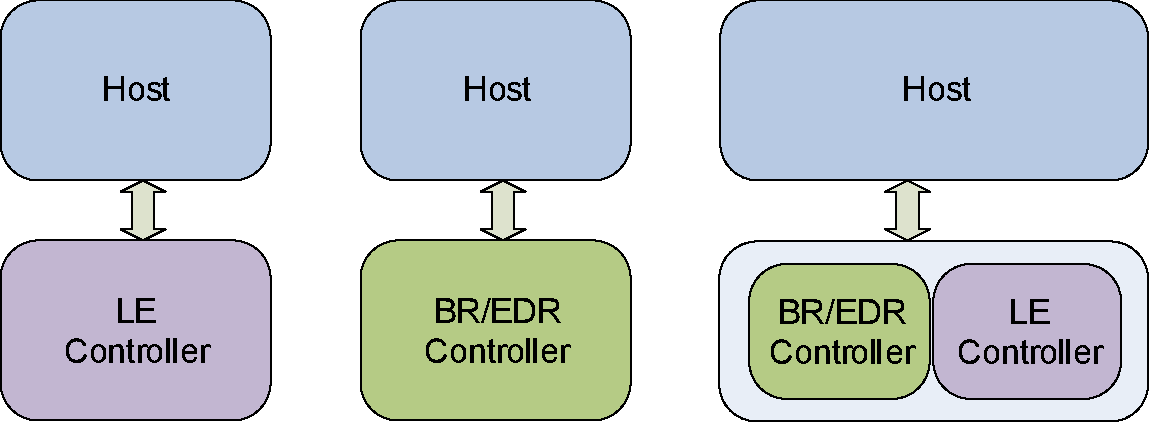
\includegraphics[width=.48\textwidth]{img/blueetooth-comunication.png}
    \caption{Descrição do funcionamento do Bluetooth. Fonte: \cite{bluetoothDocumentation}}\label{figBluetooth}
\end{figure}

O Bluetooth é implementado em duas formas: \textit{Basic Rate} (BR) e \textit{Low Energy} (LE). A diferença entre eles é que o sistema LE
possui recursos para menor consumo de corrente, baixa complexidade e custo para dispositivos cujo funcionamento tem restrição energética. O \textit{Bluetooth core system} 
organiza-se em um \textit{host} e um ou vários \textit{controllers}, onde o \textit{host} é o componente responsável 
por gerenciar os níveis acima da HCI (\textit{Host Controller Interface}) e abaixo dos perfis de aplicação externos ao protocolo. Por outro lado, o \textit{controller} 
lida com as camadas inferiores da pilha Bluetooth, como o controle do \textit{hardware} no envio e recebimento de sinais via ondas de rádio. Portanto, o 
HCI funciona como uma ponte entre os dois sistemas e atribui característica modular ao processo. A Figura \ref{figBluetooth} mostra as principais configurações: um \textit{host} com um \textit{controller} LE; 
um \textit{host} e um \textit{controller} BR/EDR, com rádio, banda de base e um gerenciador de links e, por fim, um esquema de configuração que junta ambas as implementações de Blueetooth para o dispositivo atuar inerente 
ao modo de implementação dos dispositivos alvo de conexão \cite{bluetoothDocumentation}.

\subsection{HTTP}

O HTTP (em inglês, \textit{HyperText Transfer Protocol}) é o protocolo pertencente à camada de aplicação responsável por definir a estrutura de mensagens HTTP e a forma do programa cliente e do programa servidor 
trocarem informações. O protocolo obedece à arquitetura cliente-servidor, ou seja, o cliente (geralmente um navegador Web) envia uma requisição ao servidor, que deverá processá-la e responder com um resultado, denominado resposta. O HTTP é um protocolo extensível, pois 
as solicitações de recursos poder ser realizadas em diversos formatos, como mídias, textos, áudios e muitos mais. A identificação na web de cada recurso é realizada pelo conceito de URL (em inglês, \textit{Uniform Resource Locator}), responsável por identificar de maneira única um objeto na internet \cite[pp. 72]{redeskurose2010}

Sobre o padrão de mensagens, o protocolo HTTP define o conjunto de requisição e resposta. Na mensagem de requisição, temos o elemento
chamado \textbf{método}, esse campo define qual a ação que o usuário deseja executar, sendo comum o uso de verbos
como GET, POST, HEAD, PUT e DELETE. Por exemplo, ao realizar o preeenchimento de um formulário de cadastro do site, o
navegador web realiza uma requisição do tipo POST ao servidor, pois sua intenção é a criação de um recurso,
neste caso, a nova conta. A ação é executada sobre um \textbf{caminho} único, que corresponde à organização interna dos recursos 
dentro do servidor, por exemplo, as informações sobre produtos estão no caminho ``/product''. O \textbf{cabeçalho} contém informações como: preferência de linguagem do objeto cliente,
credenciais de acesso para autenticação e autorização, tipo de conteúdo na mensagem, entre outros. Por fim, o último campo é o \textbf{corpo da mensagem}, 
onde ficam armazenados os dados \cite[pp. 77]{redeskurose2010}.

\begin{figure}[ht]
    \centering
    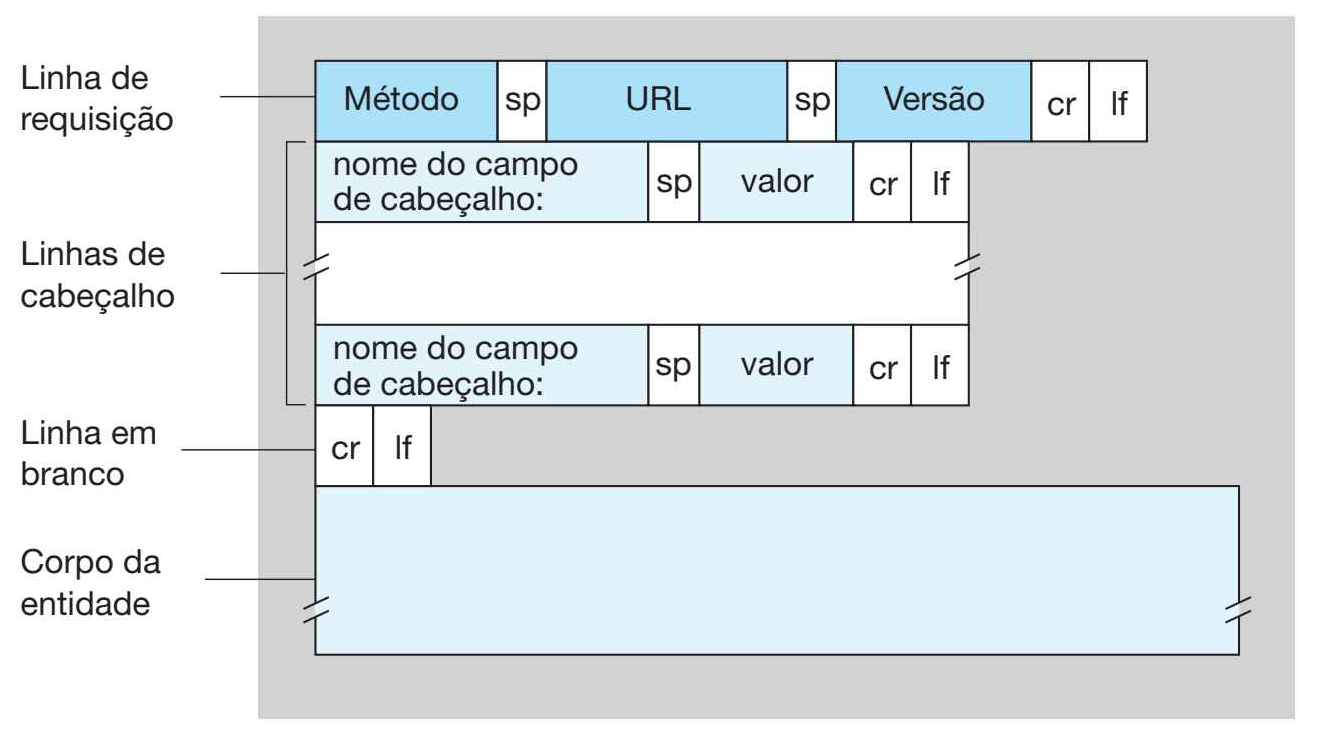
\includegraphics[width=.55\textwidth]{img/mensagem-http-solicitação.png}
    \caption{Padrão de mensagem de solicitação HTTP. Fonte: \cite{redeskurose2010}}\label{figMessageRequest}
\end{figure}

A mensagem de resposta é constituída de 3 componentes principais: linha de estado, linha de cabeçalho e corpo de entidade. Na \textbf{linha de estado}, um campo
interessante é o \textit{status code}, número pré-definido que indica se o resultado da requisição foi bem-sucedido, ou não, assim como o motivo. No \textbf{cabeçalho}
são adicionadas pelo servidor informações como o tipo do objeto e seu tamanho em bytes. Por último, o \textbf{corpo da mensagem} em si, contendo os dados solicitados \cite[pp. 78]{redeskurose2010}.

\begin{figure}[ht]
    \centering
    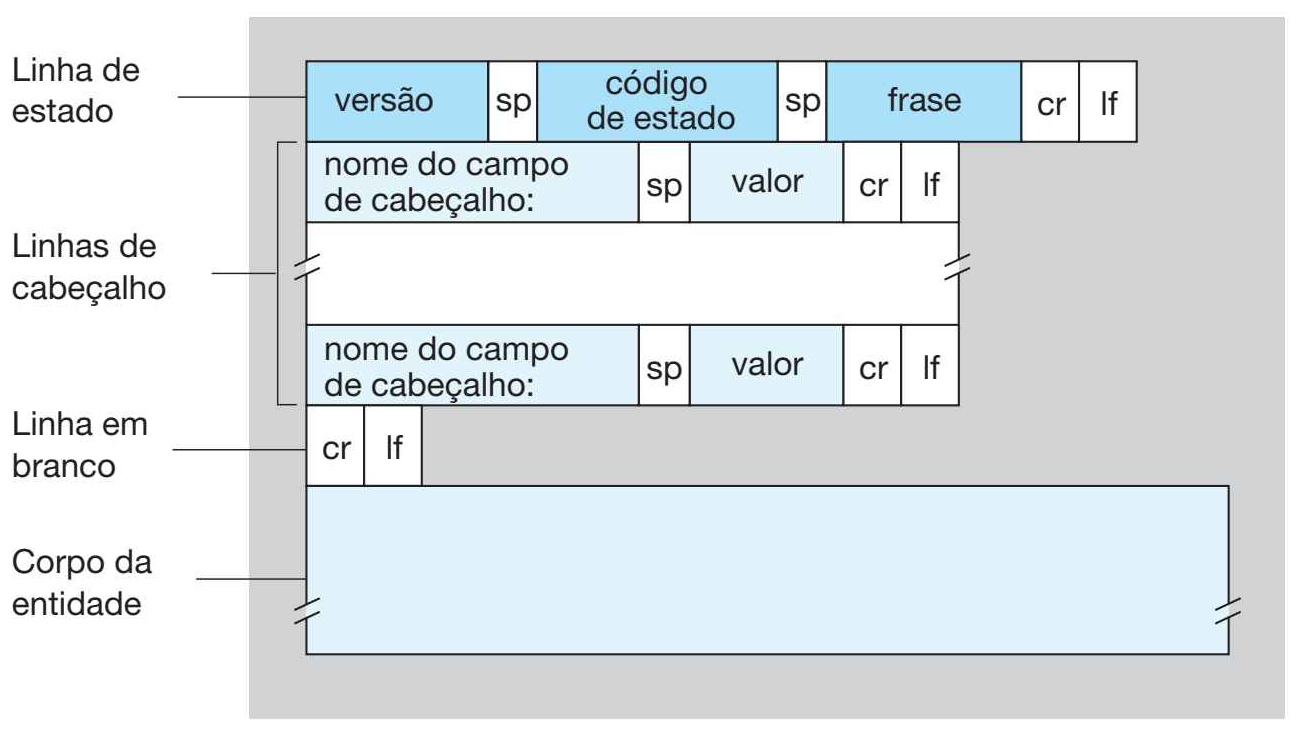
\includegraphics[width=.55\textwidth]{img/mensagem-http-resposta.png}
    \caption{Padrão de mensagem de resposta HTTP. Fonte: \cite{redeskurose2010}}\label{figMessageResponse}
\end{figure}

Dessa forma, o padrão HTTP assegura, independente de tecnologia, interação e comunicação entre clientes e servidores em todas as 
etapas de comunicação. A internet é um grande exemplo de sistema em módulos, contribuindo para o desenvolvimento de aplicações web e 
interoperabilidade nos mais diversos sistemas de computação.

\section{Desenvolvimento de aplicativos Android}

O Android possui uma extensa documentação, fornecendo os fundamentos para o desenvolvimento de 
aplicativos de alta qualidade e resilientes. Portanto, essa seção abordará as melhores práticas e recomendações
de arquitetura para a construção de aplicativos. Tais práticas envolvem o profundo
conhecimento de componentes de aplicativo, fluxos de trabalho e ciclo de vida da camada de visualização. Ao seguir uma arquitetura, 
o desenvolvedor de \textit{software} consegue melhorar sua produtividade e a qualidade de entregas, pois uma base de código aderente ao 
padrão escolhido facilita a manutenção, o desenvolvimento de novas funcionalidades e promove a colaboração entre equipes \cite{google-developers-guideline}.

\subsection{Recomendação de Arquitetura}

Um princípio muito usado na área de desenvolvimento de \textit{software} é o chamado \textit{separation of concerns}, ou separação de responsabilidades. Esse conceito, no ecossistema Android,
atua na divisão do sistema em partes menores, específicas para uma determinada função e com objetivo bem definido. Por exemplo, não misturar lógica de 
negócio ou acesso aos dados na camada de visualização (UI), tornando-a  responsável apenas pela interação com o usuário e renderização de componentes nativos. Diante disso, a documentação recomenda a separação em (pelo menos)
duas camadas principais: \textit{UI} e \textit{Data}. A camada de \textit{UI} é responsável por exibir os dados do aplicativo, refletindo a mudança na tela em resposta às
interações do usuário (como cliques ou pressionamento de botões) ou a eventos externos (como a resposta de uma requisição de rede). Por sua vez, a camada \textit{Data} fornece à camada de \textit{UI} 
um acesso simplificado aos dados, além de abrigar a lógica de negócio e o gerenciamento adequado de cada tipo de dado. Opcionalmente, pode-se adicionar uma terceira camada entre as duas, chamada de \textit{Domain Layer}.
Sua função é intermediar a comunicação entre as camadas, abstraindo chamadas e eventos em um único lugar \cite{google-developers-guideline}.

\begin{figure}[ht]
    \centering
    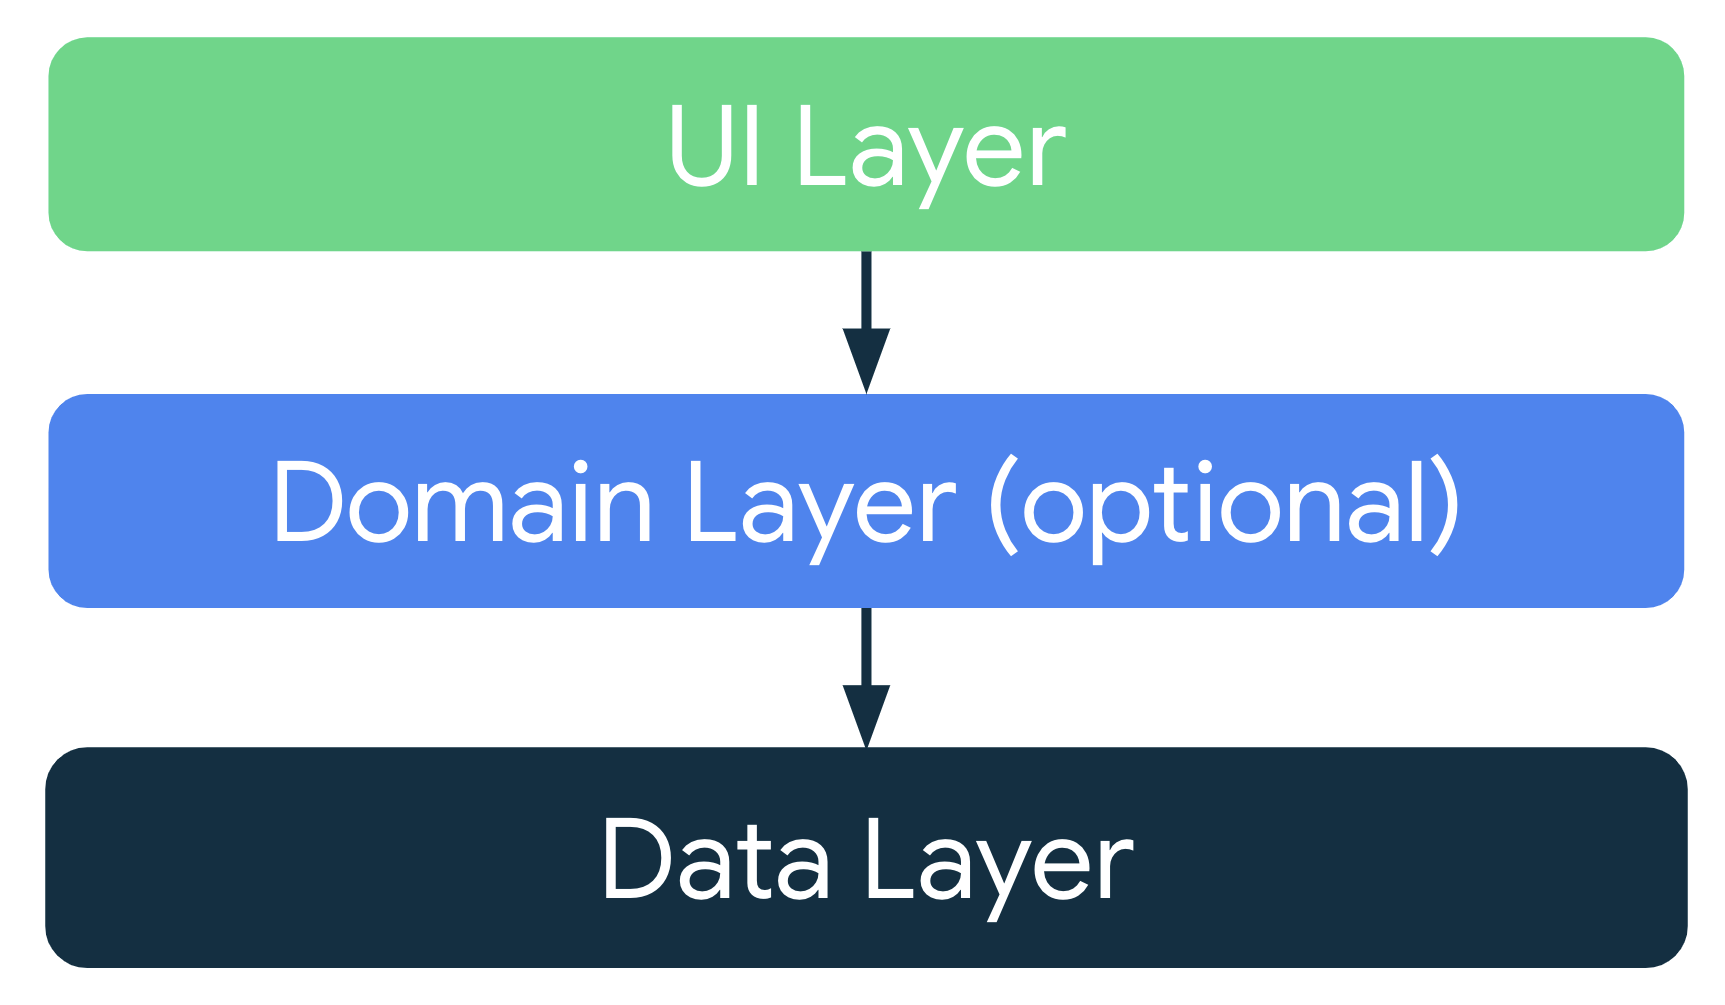
\includegraphics[width=.63\textwidth]{img/app-android-layers.png}
    \caption{Camadas de arquitetura (App). Fonte: \cite{google-developers-guideline}}\label{figAppLayer}
\end{figure}

\subsection{Ciclo de vida da atividade}\label{ciclo-de-vida}

O \textit{Activity lifecycle} (ciclo de vida de uma atividade) descreve todos os estados pelos quais uma \textit{activity} passa, do momento em que é criada
até quando é destruída. Uma \textit{activity} é uma classe Java que fornece uma janela para o aplicativo desenhar sua interface de usuário, pois um projeto Android 
inicia sempre com uma \textit{activity}. O seu ciclo de vida passa por cinco etapas: 
\textit{initialized}, \textit{created}, \textit{started}, \textit{resumed}, \textit{destroyed}. A seguir, será explicado em detalhes
cada transição de estado e o seu significado.

\begin{figure}[ht]
    \centering
    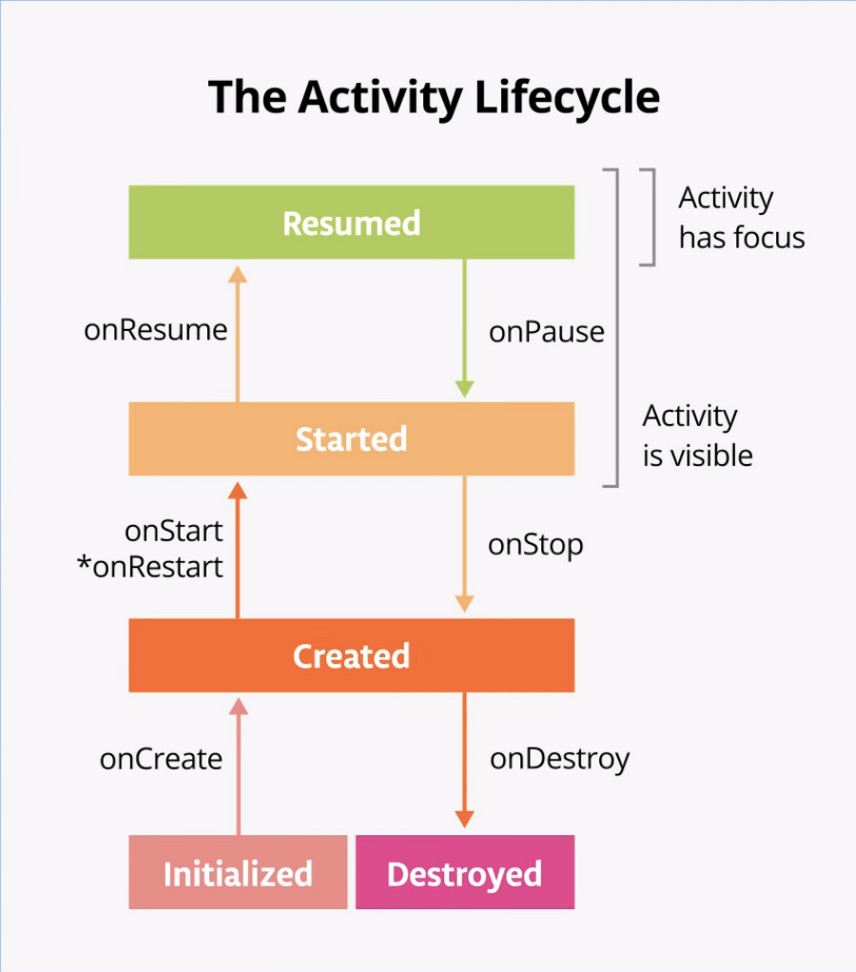
\includegraphics[width=.44\textwidth]{img/activity-lifecycle.png}
    \caption{Ciclo de vida de uma \textit{activity}. Fonte: \cite{google-developers-activity-lifecycle}}\label{figActivityLifeCycle}
\end{figure}

Quando a \textit{activity} é criada pelo sistema, o estado \textit{created} é ativado. Nesse estágio, os recursos da interface gráfica 
são inicializados, porém, a janela ainda não está disponível ao usuário. A partir do estado \textit{started}, os componentes da \textit{activity} são exibidos e a tela se torna visível, porém sem interação.
O estado \textit{resumed} é o aplicativo em primeiro plano, recebendo interações com o usuário em pleno exercício de suas funções. No entanto, se o usuário realizar uma ação que tire 
o foco do aplicativo (como verificar um e-mail após receber uma notificação), a \textit{activity} entrará no estado de pausa (paused).
Caso o usuário volte ao aplicativo, a \textit{activity} retoma os estados \textit{started} e \textit{resumed}, restaurando a interação. No entanto, se o usuário não retornar e a \textit{activity} for fechada, 
ela passará para o estado \textit{destroyed}, encerrando seu ciclo de vida \cite{google-developers-activity-lifecycle}.

\subsection{Arquitetura MVVM}

O Model-View-ViewModel (MVVM) é um padrão de projeto de \textit{software} criado por engenheiros da Microsoft\textsuperscript{\textregistered} 
cuja função é separar a lógica de software da configuração de interface do usuário. Além disso, esse padrão de projeto facilita a aplicação de testes de unidades e reutilização 
de código. O \textit{Model} é o componente não visual que armazena a lógica de negócio e o modelo de dados do domínio da aplicação, pois recebe e envia dados da \textit{ViewModel} 
para que ela interaja com a \textit{View}. A \textit{View} são os elementos visíveis de interação com o usuário, pois recebem entradas de dados e eventos de \textit{UI}. Por fim, a
\textit{ViewModel} implementa propriedades e funções para que a \textit{View} se associe aos dados e receba eventos de notificação para renderizar atualizações na camada de \textit{Model}, pois
sua ação é desacoplar o código entre os dois componentes \cite{mvvm-documentation}.

\begin{figure}[ht]
    \centering
    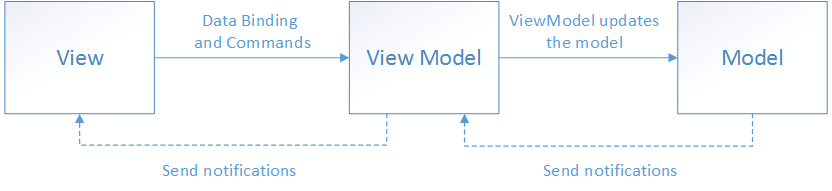
\includegraphics[width=.87\textwidth]{img/mvvm-pattern.png}
    \caption{Arquitetura MVVM. Fonte: \cite{mvvm-documentation}}\label{figMVVM}
\end{figure}

No Android, a \textit{ViewModel} possui o papel de persistência de dados quando ocorre mudança 
de estado na tela. Essas mudanças de estado são dinâmicas, como a rotação de tela ou troca de aplicativo após notificação, e, por isso, 
podem resultar em perda de dados armazenados em variáveis ou componentes visuais. A classe \textit{ViewModel}, fornecida pelo próprio 
\textit{Framework} Android, é desenvolvida para manter os dados resilientes às mudanças da interface gráfica, garantindo que informações significativas, como entradas de 
formulário e respostas de um \textit{backend}, permaneçam preservados durante a recriação da tela e componentes. Todo \textit{ViewModel} é gerenciado por um objeto 
que implementa a interface \textit{ViewModelStoreOwner}, pois seu estado é preservado durante os estados de \textit{paused}, \textit{stoped} e \textit{started} do seu \textit{Owner}, sendo destruído
juntamente com a tela, porém fechando todas suas operações com segurança. Portanto, ele funciona como um intermediário entre os dados (\textit{model}) e
os elementos visuais (\textit{view}), aderente às especificidades do ciclo de vida de uma aplicação android \cite{google-developers-viewmodel}.

\section{ESP32}

ESP32 é uma família de microcontroladores desenvolvida pela empresa Espressif Systems rica em recursos como conectividade Wi-Fi e Bluetooth projetado para aplicações de IoT. 
Está presente em soluções de automação, por apresentar vantagens como: design robusto, ao poder operar entre diferentes níveis de temperatura; 
baixo consumo de energia, onde a placa dispõe de recursos modernos como modos de baixo consumo de energia e controle dinâmico; interface de fácil 
integração com outros componentes eletrônicos e PCBs; assim como um poderoso chip integrado que atua como processador para outros sistemas de automação, 
tanto no contexto industrial quanto residencial. Restrito não somente ao \textit{hardware}, o projeto conta com uma enorme variedade 
de projetos de código aberto, incluindo bibliotecas, ferramentas, IDEs e SDKs para a construção de soluções IoT usando a placa de desenvolvimento embarcado esp32 \cite{esp32-espressif-documentation}. 

\begin{figure}[ht]
    \centering
    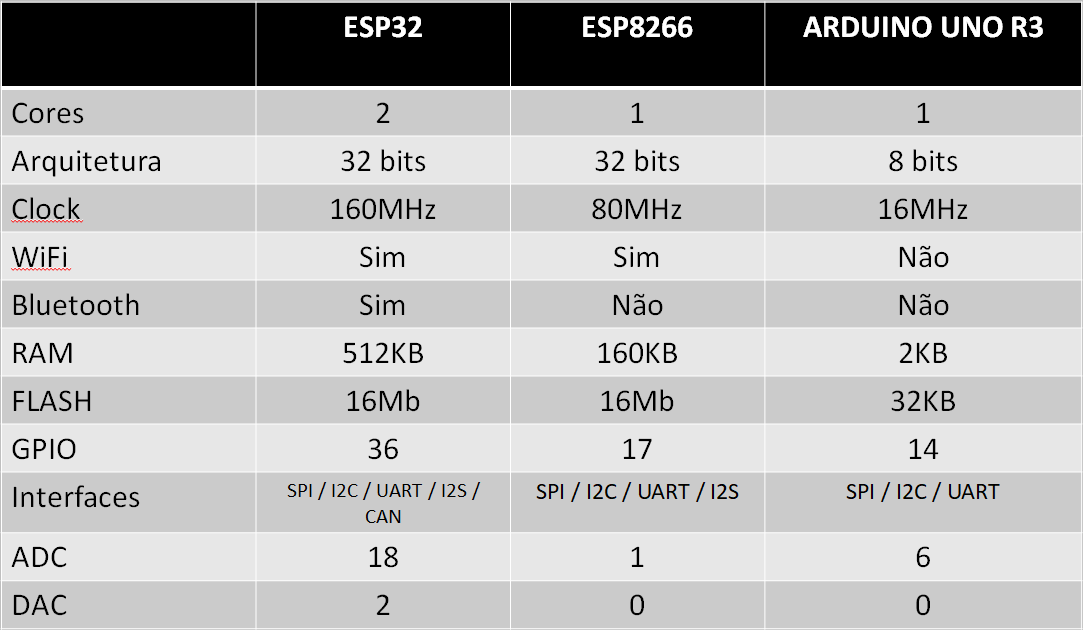
\includegraphics[width=.57\textwidth]{img/esp32-comparation-table.png}
    \caption{Comparativo entre placas de desenvolvimento. Fonte: \cite{esp32-comparation-table}}\label{figTableEsp}
\end{figure}

De acordo com a tabela, o esp32 é \textbf{dual-core}, ou seja, possui dois processadores, tem Wi-Fi e Bluetooth 
integrados e executa programas de 32 bits com memória RAM de 512KB. Portanto, a escolha do esp32 para o desenvolvimento 
do trabalho tem fundamento na robustez do dispositivo em relação aos outros citados, por permitir rodar programas maiores e lidar com mais variáveis simultaneamente (paralelismo), 
essencial para sistemas embarcados que lidam com grandes volumes de dados ou que necessitam de respostas rápidas, sendo esse o caso do sistema em construção. 

\section{Exposição ao monóxido de carbono: riscos e consequências}

O monóxido de carbono (CO) é um gás tóxico, incolor e inodoro, que resulta da combustão incompleta. A intoxicação por esse gás ocorre porque ele se liga preferencialmente à hemoglobina, a proteína 
responsável pelo transporte de oxigênio no sangue, impedindo a distribuição adequada de oxigênio pelo corpo. Como consequência, a hemoglobina se 
torna incapaz de liberar o oxigênio eficientemente nos tecidos, levando a níveis tóxicos de monóxido de carbono no sangue. Isso provoca um aumento na ventilação 
pulmonar na tentativa de compensar a falta de oxigênio, o que agrava os sintomas. O quadro clínico é inespecífico e pode incluir náuseas, aumento da 
frequência respiratória, além de, em casos mais graves, lesões cerebrais e arritmias cardíacas.

Para o diagnóstico, é importante considerar o histórico de exposição a ambientes com potencial risco, como pacientes que estiveram em locais de incêndio. Na medição 
da carboxiemoglobina (COHb) presente no sangue, o paciente pode estar assintomático ou apresentar baixos níveis da substância devido ao curto tempo de exposição, porém somente a medição da taxa de COHb é 
ineficiente para obter informação do nível de lesão causado. No entanto, um eletrocardiograma é um exame eficaz para detectar anormalidades em casos de exposição significativa ao CO. Uma vez detectada 
a intoxicação por monóxido de carbono, o paciente é submetido à terapia com suplementação de oxigênio (O\textsubscript{2}), suporte ventilatório e monitoramento de arritmias cardíacas \cite{carbon-monoxide-poisoning-varon}.

\begin{table}[h!]
    \centering
    \caption{Sintomas de Envenenamento Agudo por CO baseados nos níveis de COHb. Fonte: Retirado e traduzido de \cite{carbon-monoxide-poisoning-varon}}
    \begin{tabular}{c|c}
        \hline
        \textbf{COHb \%} & \textbf{Sintomas} \\
        \hline
        10 & Assintomático ou pode ter dor de cabeça \\
        \hline
        20 & Tontura, náusea, dispneia \\
        \hline
        30 & Distúrbios visuais \\
        \hline
        40 & Confusão, síncope \\
        \hline
        50 & Convulsões e coma \\
        \hline
        >= 60 & Disfunção cardiopulmonar e morte \\
        \hline
    \end{tabular}
\end{table}



\section{Trabalhos relacionados}\label{cap2:tabRel}

O uso de sistemas embarcados na resolução de problemas de monitoramento de ambiente e prevenção 
de acidentes possui uma ampla literatura disponível, justificando o uso de IoT em diversos setores 
presentes na sociedade, como, por exemplo, indústria, agricultura e residência. Portanto, esta seção 
discutirá soluções que compõe a base para o desenvolvimento do presente trabalho.

O trabalho de Sá possui foco no uso de dispositivos na área de IoT para a prevenção de incêndios em ambientes residenciais \cite{uea-iot-deteccao-incendio}. 
O protótipo desenvolvido é uma solução web para monitoramento de variáveis com uso do módulo NodeMCU ESP12, pois o microcontrolador envia dados de temperatura, gás inflamável e de 
fumaça por rede Wi-Fi para o backend da aplicação, feito em MySQL e PHP. No componente de \textit{hardware}, os sensores utilizados foram o BM280 (Sensor de temperatura digital) e
MQ2 (Sensor de gás/fumaça), assim como o atuador do tipo válvula para acionar o desligamento de gás de cozinha em situação de vazamento, evitando incêndio ou minimizando seus efeitos.

No contexto de proteção e acomodação dos componentes eletrônicos, foi confeccionado um \textit{case} personalizado por impressão 3D, o que conferiu acabamento 
e proteção ao protótipo. A autora também desenvolveu uma placa de circuito impresso (PCB), onde montou os sensores, atuadores e a conexão com o microcontrolador. Por fim, realizaram-se 
diversos testes e simulações, incluindo a simulação de fumaça, em que o dispositivo foi colocado na caixa com fumaça confinada, além de testes com variação de temperatura e queima de papel para acionamento do alarme. 

Semelhante ao anterior, o trabalho intitulado ``Indoor Air Quality Monitoring on AWS Using MQTT Protocol'' \cite{iot-monitoring-on-aws} mostra o desenvolvimento de um módulo de monitoramento da qualidade do ar 
em ambientes internos utilizando o protocolo MQTT e serviços da AWS. O módulo proposto utiliza sensores para medir a qualidade do ar interno, incluindo CO\textsubscript{2}, O\textsubscript{2} e poeira, com os dados sendo enviados e armazenados na 
nuvem para uma visualização em tempo real. O sistema alerta o usuário caso a qualidade do ar seja inadequada. Na arquitetura utilizada, os microcontroladores ficam espalhados 
pelo ambiente e enviam seus dados para o dispositivo central (\textit{Raspberry Pi}), pois o computador têm acesso ao servidor da AWS IoT e envia os dados coletados via protocolo MQTT.

No trabalho \textit{AirWorld} \cite{UFAMAirWorld}, a solução proposta é um aplicativo móvel informativo de qualidade do ar para ambientes públicos, pois 
sua interface informa dados do ambiente atual e orienta a prática de atividades físicas ou lazer. Os sensores utilizados foram o DHT11 para umidade do ar e temperatura, MQ7 para identificação do gás monóxido de 
carbono e, por último, o MQ-135 para dióxido de carbono, alcóol e outras substâncias tóxicas. Portanto, na arquitetura os dados são lidos pelo microcontrolador 
\textit{Lora ESP32 Heltec}, que envia para o \textit{Firebase} armazenar e exibir os dados no aplicativo Android. 

Além disso, o projeto possui tela de ajuda. A interface oferece ao usuário conhecimento sobre a qualidade do ar, poluentes que afetam sua composição e diretrizes de órgãos como a OMS sobre 
como identificar níveis de poluição com base nos parâmetros medidos pelo protótipo de \textit{hardware}. Portanto, a solução demonstra preocupação com às necessidades públicas, pois ao integrar 
no aplicativo os dados de ambiente em tempo real e informativos sobre saúde, o sistema promove conscientização e segurança nas práticas diárias de atividades físicas.

O protótipo construído no ``Intelligent based novel embedded system based IoT enabled air
pollution monitoring system'' \cite{tbRelacionado4NovelEmbeddedSystem} abordou o uso de \textit{hardware} e \textit{software} na implementação 
de uma solução para monitoramento da poluição ar usando o conceito de \textit{fog computing}, ou seja, computação em névoa. De acordo com os autores, o conceito de 
\textit{fog computing} é uma estratégia adotada para o dispositivo de IoT responsável pela coleta dos dados também possuir a ação de processamento do grande volume de variáveis coletados e, 
em seguida, enviar para o servidor na nuvem uma representação geral do estado, pois reduz a latência e economiza banda de rede.

O funcionamento do projeto é estruturado em três camadas principais: \textit{device}, \textit{fog} e \textit{cloud}. Na camada \textit{device}, 
a unidade de processamento central é um \textit{Raspberry Pi}, que atua como controlador principal. Em relação à \textit{fog layer}, estão os microcontroladores ESP 8266, responsáveis por receber, processar e 
enviar os dados dos sensores para o nó mais próximo ou a nuvem diretamente. O nó foi projetado para uso de seis sensores, sendo eles: GP2Y1014AU0F, DSM501, MQ-7, GSNT11, SO2-AF,
e MiCS2610-11, permitindo monitorar gases como $PM_{10}$, ${PM_{2.5}}$, CO, $NO_{2}$, $SO_{2}$ e $O_{3}$. No entanto, a adição do DHT11 para medição de temperatura e umidade do ar é justificada 
pela dependência que alguns sensores de gás possuem em relação à temperatura, no processo de calibração. A energia é fornecida pela bateria de 9V, onde o módulo de controle converte a tensão para 5V e 3V, conforme a 
necessidade de cada componente. Na \textit{cloud}, o servidor HTTP fornece APIs para os clientes consultarem todos os dados de qualidade do ar, por exemplo, o aplicativo Android com 
gráficos das medições de cada variável medida e o histórico do mês.

O trabalho acadêmico ``Automação residencial de monitoramento de gás por meio da plataforma Arduino e IOT'' \cite{sistema-antivazamento} teve como objetivo descrever as etapas de implementação e resultados alcançados de um sistema de automação 
residencial inteligente para monitoramento e alerta de vazamento de gás utilizando a Internet das Coisas (IoT). O sistema consiste em um microcontrolador Arduino UNO 
conectado a um sensor de gás MQ-5 e um módulo bluetooth HC-05, que envia os dados para um aplicativo Android desenvolvido na plataforma Android Studio.

Por fim, o estudo da usabilidade do aplicativo ``Ecampus Aluno'' da Universidade Federal do Amazonas \cite{ufam-design} é a principal referência para o 
teste da interface do protótipo apresentado como proposta de solução para o monitoramento do ar. De acordo com Marilis (2022), ``este trabalho tem por objetivo avaliar 
a usabilidade da interface do aplicativo institucional eCampus aluno, da Universidade Federal do Amazonas (UFAM), a fim de propor uma otimização da interface para 
melhor eficácia de uso dos serviços fornecidos pela instituição''. Portanto, os alunos participaram de um primeiro questionário para 
identificar os usuários do aplicativo e as principais dificuldades enfrentadas, pois a proposta de um novo design 
foi elaborada com base nos resultados obtidos. Assim, o projeto foi submetido ao teste de usabilidade e outra avaliação para realizar a comparação com a versão oficial da
universidade. 

Apesar dos exemplos de trabalhos já existentes na perspectiva de sistemas de monitoramento do ar e gases tóxicos, a solução deste trabalho de conclusão de curso diferencia-se na comunicação e envio de dados com acesso à internet ou não, além do envio de notificações 
baseado na quantidade de monóxido de carbono atual do ambiente, que informa os efeitos de exposição no organismo. Além dos aspectos mencionados, o sistema possui foco na interatividade do usuário doméstico, pois o processo de configuração do protótipo físico é
simplificado, análogo ao da instalação de um roteador de internet.

Outro destaque é o aplicativo Android para visualização dos dados em tempo real, que proporciona praticidade e controle em situações de risco, ao possibilitar o acompanhamento contínuo 
sem necessidade de dispositivos adicionais, garantindo ao usuário uma maior segurança e controle sobre a qualidade do ar em sua residência. Portanto, a solução proposta no contexto deste trabalho é voltada para o ambiente residencial, porém seu uso é adaptável facilmente a outros ambientes \textit{indoor}, como escritórios corporativos ou hospitais. 